\documentclass[conference]{IEEEtran}
\IEEEoverridecommandlockouts
% The preceding line is only needed to identify funding in the first footnote. If that is unneeded, please comment it out.
\usepackage{cite}
\usepackage{amsmath,amssymb,amsfonts}
\usepackage{algorithmic}
\usepackage{graphicx,subcaption}
\usepackage{textcomp}
\usepackage{xcolor}
\def\BibTeX{{\rm B\kern-.05em{\sc i\kern-.025em b}\kern-.08em
    T\kern-.1667em\lower.7ex\hbox{E}\kern-.125emX}} 

\usepackage[]{footmisc}
\usepackage{hyperref}
\usepackage{bm}
\begin{document}
\title{Classifying car images in the TCC Dataset\\
\thanks{Term project for ENSC 813. Spring 2020. SFU.}
}

\author{\IEEEauthorblockN{Ashiv Hans Dhondea}
\IEEEauthorblockA{\textit{Department of Engineering Science} \\
\textit{Simon Fraser University}\\
Burnaby, BC, Canada \\
hdhondea@sfu.ca}
}

\maketitle

\begin{abstract}
In order to analyze vehicular traffic in urban areas, transportation management services need to perform vehicle classification. Fine-grained vehicle classification aims to classify the make, model and the year of a vehicle from images. State-of-the-art approaches exploit vast datasets, deep convolutional neural networks and domain-specific knowledge for this task. Coarse-grained vehicle classification aims to do either binary or multi-class vehicle classification according to a single attribute. In this work, we implement, train and evaluate a number of convolutional neural networks to classify cars according to their make. We make use of the recent \textit{The Car Connection} dataset, we report on problems due to the lack of maturity of the dataset and we discuss solutions which we developed to mitigate these issues. Without incorporating domain-specific modifications, we experiment with data augmentation, k-fold cross-validation and ensembling. With the latter, we achieve a classification accuracy of at least $92\%$ on binary vehicle classification tasks and at least $90\%$ on multi-class vehicle classification tasks.
\end{abstract}

\begin{IEEEkeywords}
convolutional neural network, image classification, binary classifier, multi-class classifier, vehicle classification, vehicle analysis, traffic analysis, coarse-grained vehicle classification.
\end{IEEEkeywords}

\section{INTRODUCTION} \label{intro}
Vehicle classification from images finds application in the field of transportation management services and in forensic investigation. Fine-grained vehicle classification aims to classify the make, model and the year of a vehicle from images. Coarse-grained vehicle classification, on the other hand, aims to classify car images according to a single attribute, such as the make as investigated in this work. The main challenge in both cases is that the intra-class visual variation is higher than the inter-class variation. For instance, a Ford hatchback will look more similar to a Volkswagen (i.e. a different class) hatchback than to a Ford sedan (same class). To distinguish between cars of different brands, people rely on the badges (emblems), lettering, and unique design cues (e.g. kidney grille on BMWs, the Scudetto grille on Alfa Romeos, hood ornaments on Rolls-Royces and Mercedes-Benz cars, and the Hofmeister kink on rear passenger windows in BMWs). These domain-specific features can be incorporated into computer vision models to assist in the learning process. However, due to the time constraints, of this project, it was not possible for us to implement such sophisticated features.
A secondary challenge to vehicle identification is that images are taken from multiple viewpoints. 

This paper describes the architecture, training, validation and testing of a few convolutional neural networks (ConvNets) models to perform binary classification and multi-class classification of car images between brands. The goal is to provide a benchmark for classification of images according to car brands with the TCC dataset. 

This paper is organized as follows: Section \ref{section:related} reviews the relevant literature on vehicle classification and image classification. Section \ref{section:data} describes in detail the dataset used in this work. Section \ref{section:methods} discusses the architecture of the ConvNets implemented in this work. Section \ref{section:experiments} describes how experiments were run to assess the performance of the methods elaborated in the previous section. Finally, Section \ref{section:conclusion} summarizes the results of the paper and provides recommendations for future work.

\section{Related work} \label{section:related}
Following the victory of Pierre Sermanet's Convolutional Neural Network-based solution in Kaggle's famous Cats versus Dogs competition \cite{kagcatdog}, Convolutional Neural Network (ConvNet or CNN)-based approaches have become an almost \textit{de facto} approach in research and development work on image classification, Indeed, ConvNet-based approaches have achieved state-of-the-art accuracy in several object classification tasks \cite{simonyan2014very}. 
%For fine-grained vehicle classification tasks, Krause \textit{et al.} have developed classifiers which are part-based rather than CNN-based  in \cite{KrauseStarkDengFei-Fei3DRR2013}. The part-based approach is rooted in 3-dimensional object representation

Most research papers on vehicle classification have focused on fine-grained vehicle classification according to a set of attributes rather than a single attribute such as the brand. In \cite{7744550}, Fang, Zhou and Du developed an approach which combines part-based methods and ConvNets to do fine-grained classification of vehicle images according to make and model. In \cite{7535529}, convolutional neural networks were used to classify images between body types (truck, van, car and bus) without incorporating modifications specific to vehicles. In \cite{7891907}, a spatially weighted pooling layers was added to ConvNets to classify car images according to three attributes - make, model and year. In 2017 \cite{liu2017monza}, car images were classified according to make and model with a number of approaches: a Support Vector Machine, a one layer ConvNet and several well-known CNN architectures such as VGG16 \cite{krizhevsky2012imagenet} trained from scratch, with transfer learning or with transfer learning and fine tuning. The best results were obtained with transfer learning with GoogleNet \cite{Szegedy2015CVPR}. In 2018 \cite{valev2018systematic}, Valev \textit{et al.} have evaluated the performance of several ConvNet architectures such as VGG16 \cite{krizhevsky2012imagenet}, ResNet50 \cite{he2016deep} and DenseNet-121 \cite{huang2017densely} on the Stanford Cars-196 dataset \cite{KrauseStarkDengFei-Fei3DRR2013}. Using bounding boxes annotating the location of cars in images (provided in \cite{KrauseStarkDengFei-Fei3DRR2013}), Valev \textit{et al.} trained neural networks both from scratch and from transfer learning to classify images in 196 categories. Horizontal flipping was the most beneficial form of data augmentation since it improved the test accuracy by $2.9\%$ \cite{valev2018systematic}. Due to the small number of examples (40) available for each category in the dataset, deeper networks could not be trained from scratch to produce adequate results \cite{valev2018systematic}.

\section{Data} \label{section:data}
\subsection{Source and Exploratory Data Analysis}
The dataset used in this project was scraped from \textit{The Car Connection} website (\url{https://www.thecarconnection.com/}) by Mr. Nicolas Gervais. It contains around 60,000 images of vehicles labeled with their specifications (make, model, year, price, horsepower, etc). The GitHub repository found at \cite{githubrepo} provides links to download the data set and starter codes in Jupyter notebooks for analysis. Images in this dataset are from various viewpoints, instead of a single, common viewpoint which would facilitate the image classification task. Furthermore, cars in the images are in unconstrained poses. 

The TCC dataset lacks maturity in comparison with established datasets such as the Stanford-196 cars dataset \cite{KrauseStarkDengFei-Fei3DRR2013}. A car aficionado will notice that a large number of images are incorrectly labeled (e.g. wrong make or model). This is most likely caused by the automated web scraper extracting images from articles comparing several cars and mis-attributing all images to the first brand name and model mentioned in the article's title. Furthermore, a certain portion of the dataset consists of interior shot images, detail images focusing on a specific car part e.g. handles and outside mirrors and CAD drawings of concept cars wrongly attributed to an existing car model. Finally, some images contain more than one car, which is not desirable. All of these images have to be rejected since they may fool classifiers into giving unreliable results. The vast majority of images in the TCC dataset are $360 \times 240$ pixels. Despite the shortcomings of the TCC dataset, it was retained for the purposes of this project. Since the TCC dataset contains a few thousand images of each brand's vehicles, it was deemed to be suitable for training classifiers from scratch according to car brands. The TCC dataset has not been split into a training set and an evaluation set, in constrast to the Stanford-196 dataset. This means that a test set has to be randomly selected from the dataset in order to evaluate learning methods.

\begin{figure}[t]
    \centering
    \begin{subfigure}[b]{0.48\linewidth}        %% or \columnwidth
        \centering
        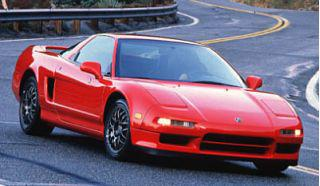
\includegraphics[width=0.96\linewidth]{Acura_NSX_2001_84_16_250_30_6_71_46_174_17_RWD_2_2_2dr_VcY.jpg}
        \caption{Correctly labeled as Acura NSX.}
        \label{fig:A}
    \end{subfigure}
    \begin{subfigure}[b]{0.48\linewidth}        %% or \columnwidth
        \centering
        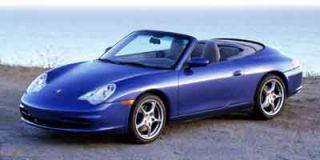
\includegraphics[width=0.96\linewidth]{Acura_NSX_2003_89_17_250_30_6_71_46_174_17_RWD_2_2_2dr_BGc.jpg}
        \caption{Incorrectly labeled as Acura NSX.}
        \label{fig:B}
    \end{subfigure}
    \caption{Both images are labeled as Acura NSX. The image on the left is correctly labeled but the one on the right (a Porsche 911 Cabriolet) is incorrectly labeled.}
    \label{fig:acura}
\end{figure}

As previously mentioned in Section \ref{intro}, the intra-class visual variation is higher than the inter-class variation in the car image classification task. Even though the cars in Figures \ref{fig:bmwx4} and \ref{fig:mercglc} are from different brands (therefore, they belong to different classes for our purposes), they are more visually similar to each other than to another vehicle from the same brand in Figure \ref{fig:bmwz4} and Figure \ref{fig:merccoupe} respectively. This is because body type (sedan, hatchback, SUV) has a stronger influence on visual appearance than brand. As can be seen from Figures \ref{fig:bmwz4} and \ref{fig:merccoupe}, cabriolets from different brands/classes are very similar to each other.

\begin{figure}[t]
    \centering
    \begin{subfigure}[b]{0.48\linewidth}        %% or \columnwidth
        \centering
        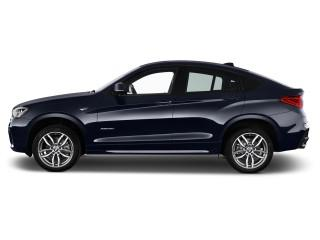
\includegraphics[width=0.96\linewidth]{BMW_X4_2015_44_18_240_20_4_74_63_184_20_AWD_5_4_SUV_zYa.jpg}
        \caption{BMW X4 image}
        \label{fig:bmwx4}
    \end{subfigure}
    \begin{subfigure}[b]{0.48\linewidth}        %% or \columnwidth
        \centering
        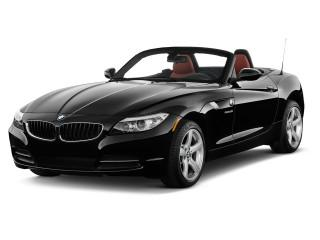
\includegraphics[width=0.96\linewidth]{BMW_Z4_2014_48_17_240_20_4_70_50_166_22_RWD_2_2_Convertible_hra.jpg}
        \caption{BMW Z4 image.}
        \label{fig:bmwz4}
    \end{subfigure}
    \caption{Visually different images of cars from the same brand (BMW).}
    \label{fig:bmw}
\end{figure}

\begin{figure}[t]
    \centering
    \begin{subfigure}[b]{0.48\linewidth}        %% or \columnwidth
        \centering
        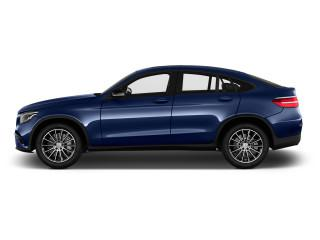
\includegraphics[width=0.96\linewidth]{Mercedes-Benz_GLC Class_2019_61_20_360_30_6_76_62_186_19_AWD_5_4_SUV_Rpc.jpg}
        \caption{Mercedes GLC image}
        \label{fig:mercglc}
    \end{subfigure}
    \begin{subfigure}[b]{0.48\linewidth}        %% or \columnwidth
        \centering
        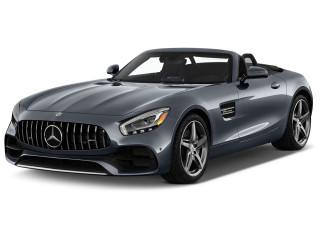
\includegraphics[width=0.96\linewidth]{Mercedes-Benz_AMG GT_2019_99_19_420_30_6_76_57_199_19_AWD_4_4_4dr_snY.jpg}
        \caption{Mercedes AMG GT image.}
        \label{fig:merccoupe}
    \end{subfigure}
    \caption{Visually different images of cars from the same brand (Mercedes).}
    \label{fig:mercedes}
\end{figure}

\subsection{Cleaning the dataset}
The raw TCC dataset had to be filtered to reject incorrectly labeled images and useless images of car parts and car interiors. To reduce the magnitude of this daunting task, images belonging to only six classes were selected and then filtered. 

\subsection{Classes used in this work} \label{cla}
As mentioned previously, six classes were selected and their images were used in experiments in this work. The distribution of brands in the manually curated dataset is shown in Figure \ref{fig:distrib}.

\begin{figure}[t]
	\centering
	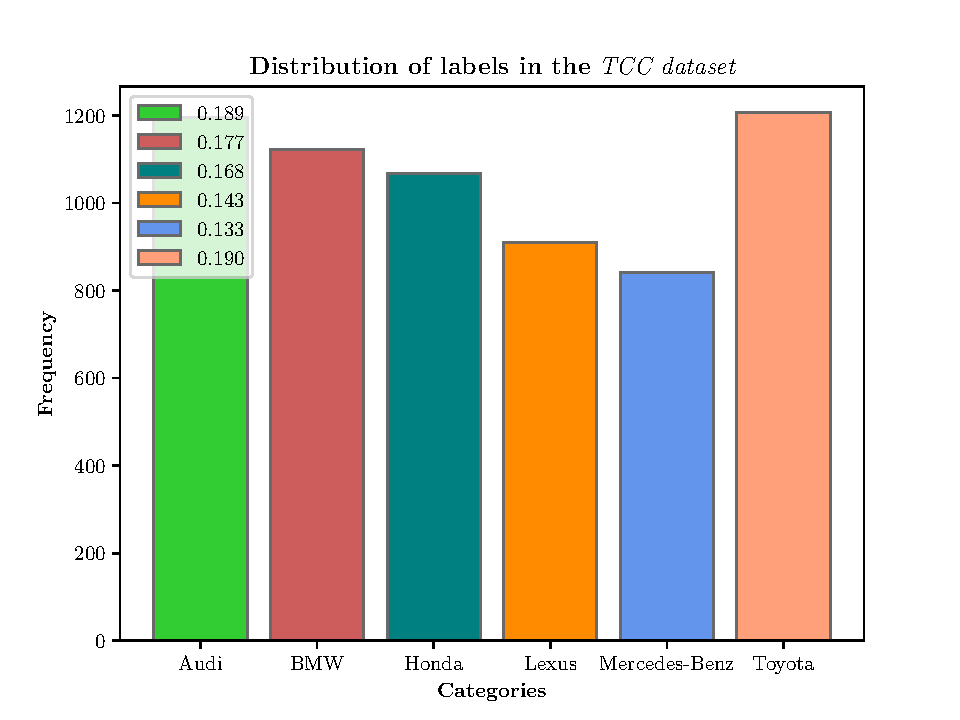
\includegraphics[scale=0.42]{main16edaootable.pdf}
	\caption{Distribution of images in the dataset in six classes. Audi, BMW, Honda and Toyota are over-represented while Lexus and Mercedes-Benz are under-represented (i.e. having a proportion less than $16.67\%$).} 
	\label{fig:distrib}
\end{figure}

The imbalance in the dataset was corrected by undersampling the over-represented examples in the images relevant to each comparison. For example, to classify Lexus versus Mercedes-Benz images, 841 Lexus images were selected at random, to match the 841 examples of Mercedes-Benz in the dataset. This ensures equal representation of both classes in the dataset used for binary classification.

\section{Methods} \label{section:methods}
Binary classification between pairs of car brands and multi-class classification between four car brands were done in this work.

\subsection{Binary classifiers}
Four convolutional neural networks were used to perform binary classification between images from pairs of car brands. Their architectures are shown in Table \ref{table:bin:method} \footnote{Ref. Table \ref{table:bin:method}: conv3x3 means $3 \times 3$ convolutional filters. ReLu means Rectified Linear Unit. mp2x2 means max pooling with a $2\times2$ window and a stride of 2. Flatten means flattening the matrix or tensor to a vector. fc64 means a layer consisting of 64 fully-connected nodes. Dropout 0.5 means dropping the weights of $50\%$ of the units. o1 means 1 output node.}. Feature learning layers make use of three or four convolutional layers with 32, 64, 128 or 256 filters of dimension $3 \times 3$. ReLu (Rectified Linear Unit) was used as activation function since it is usually employed for general image classification tasks. Max pooling with $2 \times 2$ kernels and a stride of 2 was done to provide regularization in the training process. Model 1 is the ConvNet developed by Chollet in \cite{chollet2018deep} for the Cats versus Dogs Kaggle classification challenge \cite{kagcatdog}. The architecture of this CNN is a very simplified version of the VGG16 architecture. The other three architectures are slightly less simplified versions of the VGG16 architecture. To improve on the results of Model 1, our ConvNets had to discriminate more accurately between images of different car brands. To do so, the ConvNets have to learn more features from the training set images and become more discriminative in the classification layers. Therefore, we increased the number of layers for feature learning and added more nodes in the classification stage. Model 4 differs from Model 3 in that the dropout factor decreased from 0.5 to 0.3. Even though we do not report results with deeper ConvNets in this paper, we empirically found that deeper CNNs perform significantly worse than shallower networks in the binary classification task at hand.
This is because the limited amount of examples available in the curated dataset hamstring the training of deeper ConvNets. Furthermore, the task of classifying car images between two brands is not very hard since shallow ConvNets can reach classification accuracies of upwards of $90\%$. This means that deeper ConvNets will be more prone to overfitting the training set since they attempt to fit overly complicated models to a problem which is not necessarily complicated.

\begin{table*}[t]
	\caption[ConvNet models used for the binary classification task]{ConvNet models used for the binary classification task} \label{table:bin:method}
	\centering
\begin{tabular}{| c | c | c | c | c |}
\hline
 & \textbf{Model 1} & \textbf{Model 2}  &  \textbf{Model 3} & \textbf{Model 4}\\
\hline \hline
\textbf{Feature Learning} &  32conv3x3 + ReLu - mp2x2 & 32conv3x3  + ReLu - mp2x2 & 32conv3x3  + ReLu - mp2x2 & 32conv3x3  + ReLu - mp2x2 \\
 & 32conv3x3  + ReLu - mp2x2 & 64conv3x3  + ReLu - mp2x2 & 64conv3x3  + ReLu - mp2x2 & 64conv3x3  + ReLu - mp2x2\\
 & 64conv3x3  + ReLu - mp2x2 & 128conv3x3  + ReLu - mp2x2 & 128conv3x3  + ReLu - mp2x2 & 128conv3x3  + ReLu - mp2x2\\
 & & 256conv3x3  + ReLu - mp2x2 &  128conv3x3 + ReLu - mp2x2 & 128conv3x3 + ReLu - mp2x2 \\
 \hline
 \textbf{Classification} & flatten & flatten & flatten & flatten\\
  & fc64 + Relu & fc256 + ReLu & fc256 + ReLu & fc256 + ReLu \\
  & dropout 0.5 & dropout 0.5 & dropout 0.5 & dropout 0.3\\
  & o1 + sigmoid & o1 + sigmoid & o1 + sigmoid & o1 + sigmoid \\
 \hline
\end{tabular}
\end{table*}

Model 4 differs further from Model 3 by including data augmentation for the training and validation sets. As pointed out in Section \ref{section:related}, horizontal flipping is an apt choice of data augmentation strategy. This is because many images in the TCC dataset are taken from either the right hand side or the left hand side of the vehicles.

\subsection{Multi-class methods}
For multi-class classification, the ConvNets used for binary classification were modified: the number of output nodes was increased from a single one to four, to match the higher number of classes in this task. The activation function in the last layer was changed to softmax, which is the multi-class generalization of the sigmoid activation function for logistic regression. A fifth model was developed from Model 2: in the feature learning stage, it has an additional layer consisting of 512conv3x3 + ReLu - mp2x2, in the classification stage, the dropout was decreased to 0.3 and the activation function for the four output nodes was changed to softmax. In addition, data augmentation in the form of horizontal flipping was included.

\section{Experiments} \label{section:experiments}
The TCC dataset does not have a dedicated test set on which the classification performance of different methods can be benchmarked. Therefore, in each experiment, the curated dataset was randomly shuffled and then split into a test set and a training/validation set. The validation set was used as criteria for early stopping, which is a form of regularization. The learned weights corresponding to the lowest validation loss were used when testing with the test set. Since the test set was independent from the training and validation sets, it was not contaminated by the learning process and was therefore ideal for estimating the out-of-sample performance of our ConvNets. All experiments done in this work made use of Keras \cite{keras} and the GPU version of Tensorflow. The optimizer used in all experiments was Adam and learning rates used were between 0.00001 and 0.00005. A batch size of 32 examples was used in all experiments.

\subsection{k-fold cross-validation}
To ensure that all examples in the training/validation set are used for both training and validation, we made use of 10-fold cross-validation. For each fold, we performed early stopping according to the validation loss to identify the best learned weights. With these weights, the out-of-sample performance was evaluated by testing on the test set which was held out. The accuracy on the test set was stored for each fold. By using the same seed numbers for splitting and shuffling with different ConvNets, we ensured that the exact same test set was generated for each ConvNet. This is necessary for the benchmark test to be fair.

\subsection{Ensembling the classifiers}
Normalized correlation-based ensembling was implemented to combine the strengths of the binary classifiers we developed in this work. ConvNets were trained with $66\%$ of the dataset and $17\%$ of the examples in the dataset were reserved for validation. With the best weights chosen at the minimum validation loss, the ConvNets were evaluated over the test set, which consisted of $17\%$ of the examples in the dataset. Ensembling in the form of averaging was implemented to improve the out-of-sample performance in the multi-class classification task.

\section{Results} \label{section:results}
\subsection{Binary classification}
For the 10-fold cross validation experiments, we randomly split the dataset such that $20\%$ of the examples were held out for testing while the other $80\%$ were used for training and validation with the 10-fold cross validation method. 

\begin{figure}[ht]
    \centering
    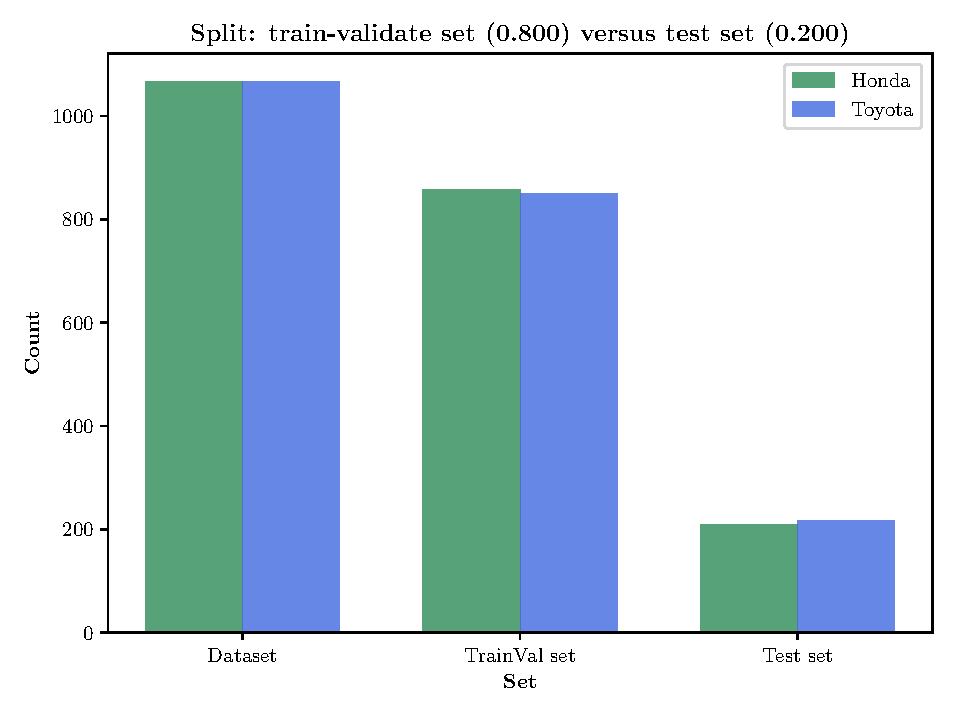
\includegraphics[scale=0.48]{main_03_binary_classification_00_Honda_Toyota_split.pdf}
    \caption{Honda v. Toyota classification: while $80\%$ of the dataset was used for training and validation, $20\%$ of the examples were held out for testing.}
    \label{fig:hondatoyo}
\end{figure}

Table \ref{table:bin:kfold} shows the average test accuracy obtained with the four CNN models over three classification tasks. These specific pairs of brands were chosen for experimentation because their vehicles have similar silhouettes in our opinion. Model 3 achieved the best accuracy for the Audi vs. BMW and the Honda vs. Toyota classification problems and had the second best accuracy for the Lexus vs. Mercedes-Benz classification task. Overall, all ConvNets achieved an accuracy exceeding $90\%$ in all three classification tasks, which is very encouraging.

\begin{table*}[t]
	\caption{Binary classification task: 10-fold Cross Validation test accuracy results with 4 ConvNets} \label{table:bin:kfold}
	\centering
\begin{tabular}{| l | c| c| c|}
\hline
\textbf{Model} & \textbf{Audi v. BMW} & \textbf{Lexus v. Mercedes}  &  \textbf{Honda v. Toyota}\\
\hline \hline
1 &  $95.6159\%$ &  $\bm{98.5163\%}$ &  $91.8033\%$ \\ \hline
2 &  $96.2422\%$ &  $97.9228\%$ &  $93.4426\%$ \\ \hline
3 &  $\bm{97.0772\%}$ &  $98.2196\%$ &  $\bm{94.3794\%}$ \\ \hline
4 &  $96.6597\%$ &  $97.9228\%$ &  $92.9742\%$ \\ \hline
\end{tabular}
\end{table*}

The Honda v. Toyota classification task ended up with the lowest classification accuracy regardless of the CNN model used. The highest classification accuracy in this task, $92.9742\%$ was $1.2365\%$ lower than the lowest classification accuracy in all other experiments. We can surmise that the consistently poorer accuracy for this task can be explained thus: perhaps these two brands produce vehicles which are very visually similar to each other, which makes the classification task harder. Apart from the Honda v. Toyota task, all of our test results show that the models we learned generalize very well out-of-sample since their test accuracy always exceeds $95\%$.

The four models are combined through ensembling to better classify car images. Figure \ref{fig:loss} shows the training and validation loss plot for Model 1 in the Lexus v. Mercedes-Benz classification task. The minimum validation loss occurred at epoch 65. This corresponded to a validation accuracy of $99\%$ as can be seen in the accuracy plot in Figure \ref{fig:acc}. Models with weights corresponding to the best validation loss were used in the ensembling process.

\begin{figure}[ht]
    \centering
    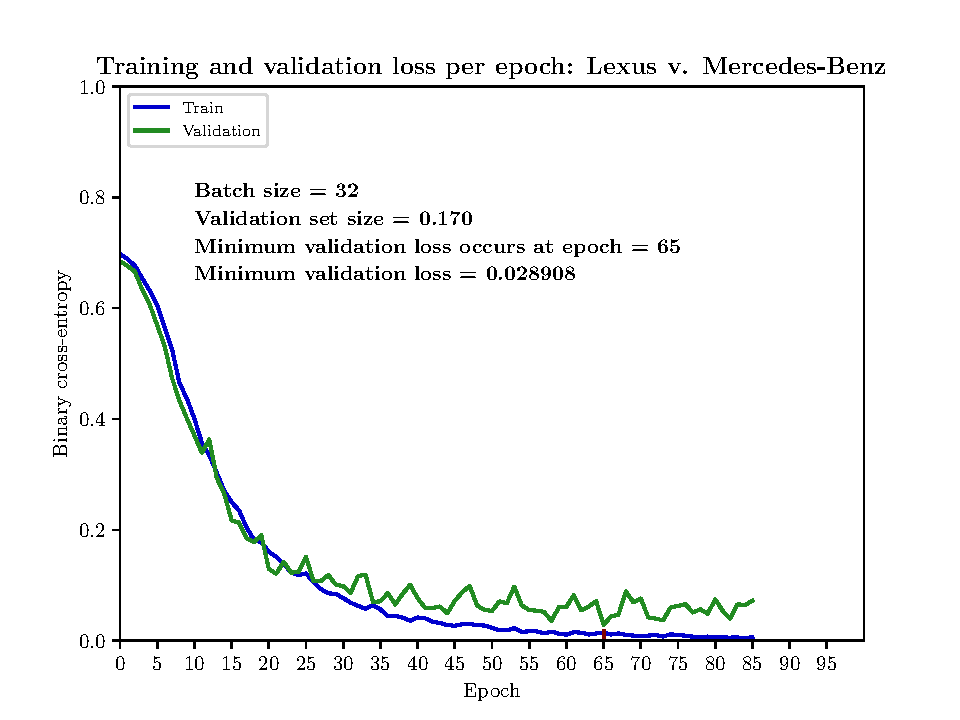
\includegraphics[scale=0.48]{main_08_binary_classification_00_Lexus_Mercedes-Benz__model_1loss.pdf}
    \caption{Binary classification with Model 1: training and validation loss per epoch}
    \label{fig:loss}
\end{figure}

\begin{figure}[ht]
    \centering
    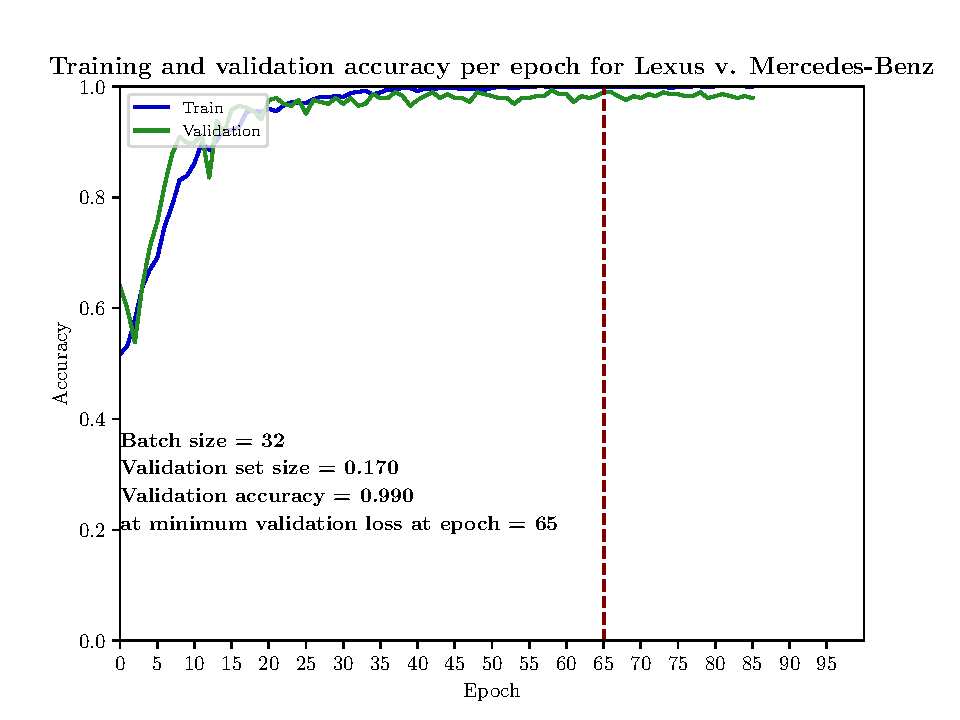
\includegraphics[scale=0.48]{main_08_binary_classification_00_Lexus_Mercedes-Benz__model_1accuracy.pdf}
    \caption{Binary classification with Model 1: training and validation accuracy per epoch}
    \label{fig:acc}
\end{figure}

The exact same training set, validation set and test set were used in experiments with the the other three models for the other classification tasks. Table \ref{table:bin:ensem} shows the test accuracy results with the four models on their own and as an ensemble through normalized correlation for the binary classification tasks. In all cases, ensembling has improved the testing accuracy by at least $0.27\%$ with respect to the individual models' accuracy.

\begin{table*}[t]
	\caption{Binary classification task: test accuracy results with 4 ConvNets and ensembling} \label{table:bin:ensem}
	\centering
\begin{tabular}{| l | c| c| c|}
\hline
\textbf{Model} & \textbf{Audi v. BMW} & \textbf{Lexus v. Mercedes}  &  \textbf{Honda v. Toyota}\\
\hline \hline
Model 1  &  $93.8575\%$ & $96.1538\%$ & $89.2562\%$\\ \hline
Model 2  &  $95.3317\%$ & $95.4545\%$ & $90.9091\%$ \\ \hline 
Model 3  &  $95.8231\%$ & $97.2028\%$ & $92.0110\%$ \\ \hline 
Model 4  &  $95.5774\%$ & $97.2028\%$ & $92.0110\%$  \\ \hline 
\textbf{Ensemble} &  $\bm{96.0688\%}$ & $\bm{97.5524}$ & $\bm{92.2865\%}$ \\ \hline
\end{tabular}
\end{table*}

The validation accuracy of $99\%$ shown in Figure \ref{fig:acc} is about $0.5\%$ higher than the test accuracy shown in Table \ref{table:bin:kfold}. This is not unusual since the out-of-sample error is usually higher than the in-sample error.

\subsection{Multi-class classification}
The multi-class classification task was done with examples from the following classes: Audi, BMW, Lexus and Mercedes-Benz. To ensure that the dataset used for learning was balanced, over-represented classes were undersampled as explained previously in Subsection \ref{cla}. Examples from the over-represented classes were randomly selected in the undersampling process. The resulting dataset has the balanced distribution shown in Figure \ref{fig:dist}.

\begin{figure}[ht]
    \centering
    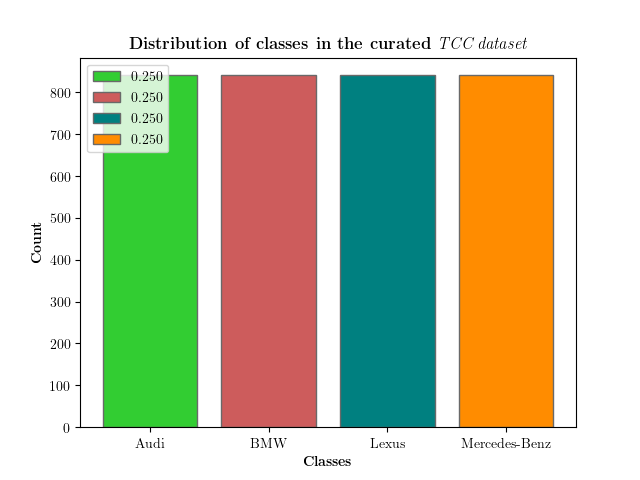
\includegraphics[scale=0.48]{main_19_multiclass_classification_00_undersampl_balanced_dataset.png}
    \caption{Distribution of classes after undersampling}
    \label{fig:dist}
\end{figure}

In a similar fashion to the ensembling experiments done in the binary classification cases, the data set was split in the following way: $66\%$ of the examples were used for training, $17\%$ were used for validation and the remaining $17\%$ were reserved for testing, as shown in Figure \ref{fig:multi}. There are slight variations in the representation of the four classes in the three subsets due to the random nature of the split. 

\begin{figure}[ht]
    \centering
    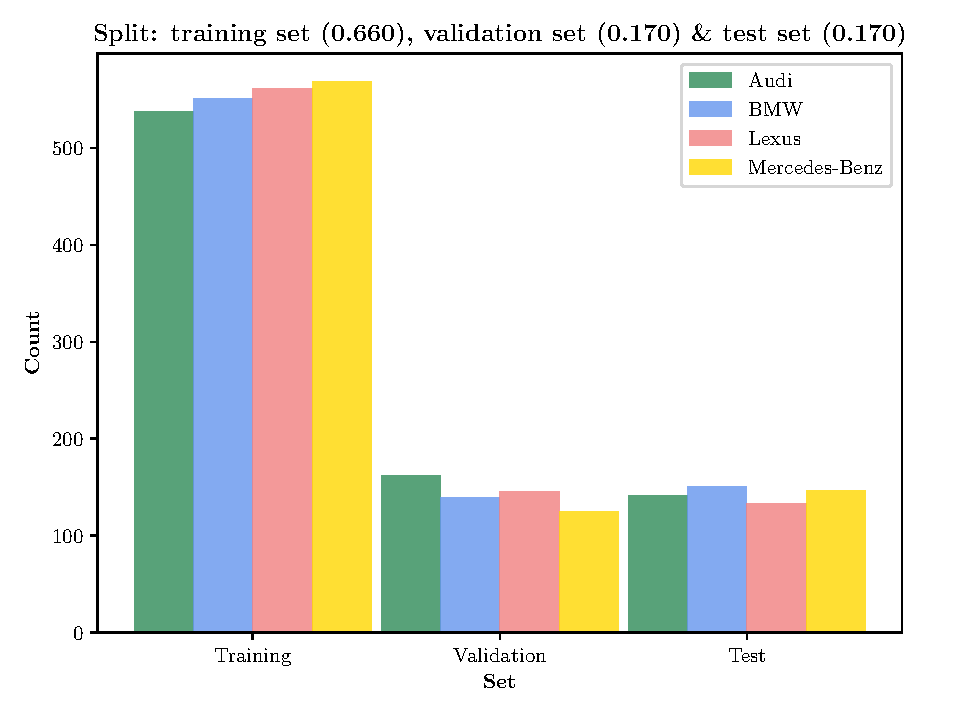
\includegraphics[scale=0.5]{main_23_multiclass_00split.pdf}
    \caption{Dataset partitioned between training, validation and test sets for the multi-class classification task}
    \label{fig:multi}
\end{figure}

Early stopping according to non-decreasing validation loss was implemented.
Figure \ref{fig:multi:loss} shows the training and validation loss plot for Model 5. The minimum validation loss occurred at epoch 172, which corresponded to a validation accuracy of $92.3\%$. 

\begin{figure}[ht]
    \centering
    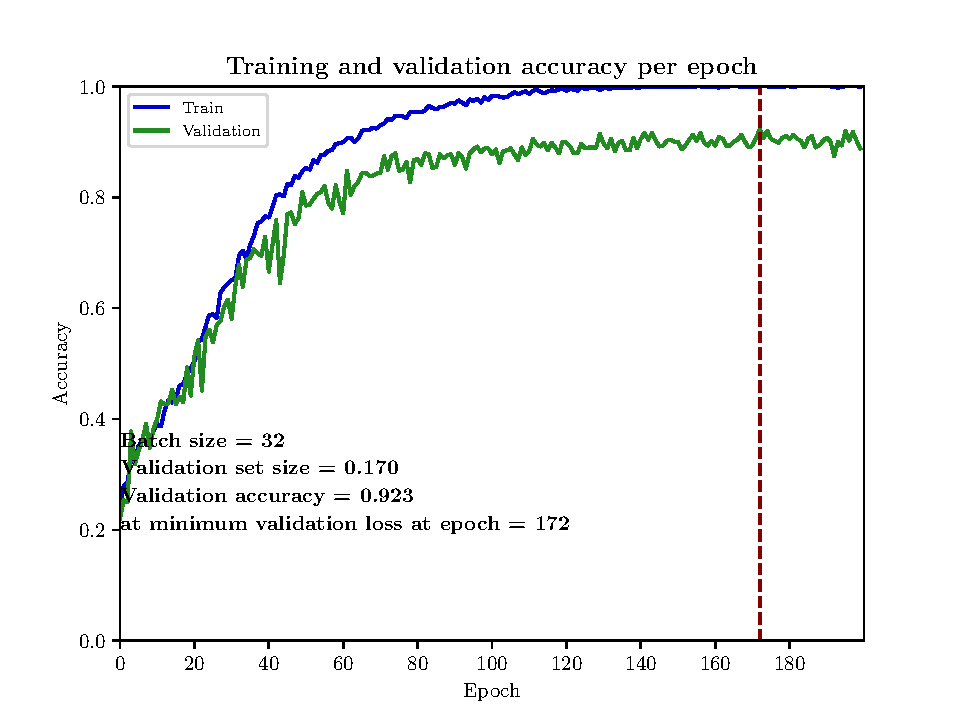
\includegraphics[scale=0.48]{main_24_multiclass_00_accuracy.pdf}
    \caption{Multi-class classification with Model 5: training and validation accuracy per epoch}
    \label{fig:multi:acc}
\end{figure}

\begin{figure}[ht]
    \centering
    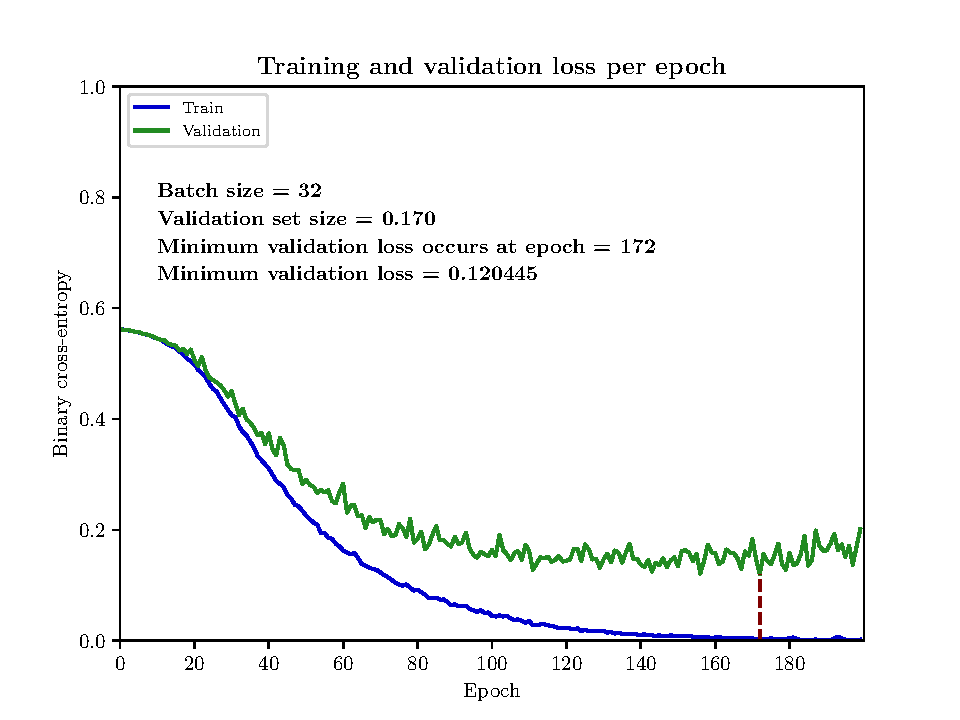
\includegraphics[scale=0.48]{main_24_multiclass_00_loss.pdf}
    \caption{Multi-class classification with Model 5: training and validation loss per epoch}
    \label{fig:multi:loss}
\end{figure}

The five models are ensembled by averaging to better classify car images among four classes. Table \ref{table:multi:ensemble} shows the test accuracy with each method. Ensembling has improved the testing accuracy by at least $1.0489\%$ compared to the individual models. Test accuracies are more than $2\%$ lower than validation accuracies in the multi-class problem. This means that the models learned have some problem generalizing out of sample, in spite of the regularization strategies we implemented such as dropout and early stopping.

\begin{table}[ht]
	\caption{Multi-class classification task: test accuracy} \label{table:multi:ensemble}
	\centering
\begin{tabular}{| l | c| }
\hline
\textbf{Model} & \textbf{Test accuracy} \\
\hline \hline
Method 1 &  $85.8392\%$ \\ \hline 
Method 2 &  $89.3357\%$ \\ \hline 
Method 3 &  $88.9860\%$ \\ \hline 
Method 4 &  $87.0629\%$ \\ \hline 
Method 5 &  $89.1608\%$ \\ \hline
\textbf{Ensemble} &  $90.3846\%$ \\ 
\hline
\end{tabular}
\end{table}

Figure \ref{fig:confmat} shows the confusion matrix with the ensemble. For each pair of actual class and predicted class, at most 10 examples from the test set were misclassified by the ensemble classifier. It is interesting to note that no Audi image was misclassified as a Mercedes-Benz image and only one of the BMW and Lexus test images were misclassified as a Mercedes-Benz image.

\begin{figure}
    \centering
    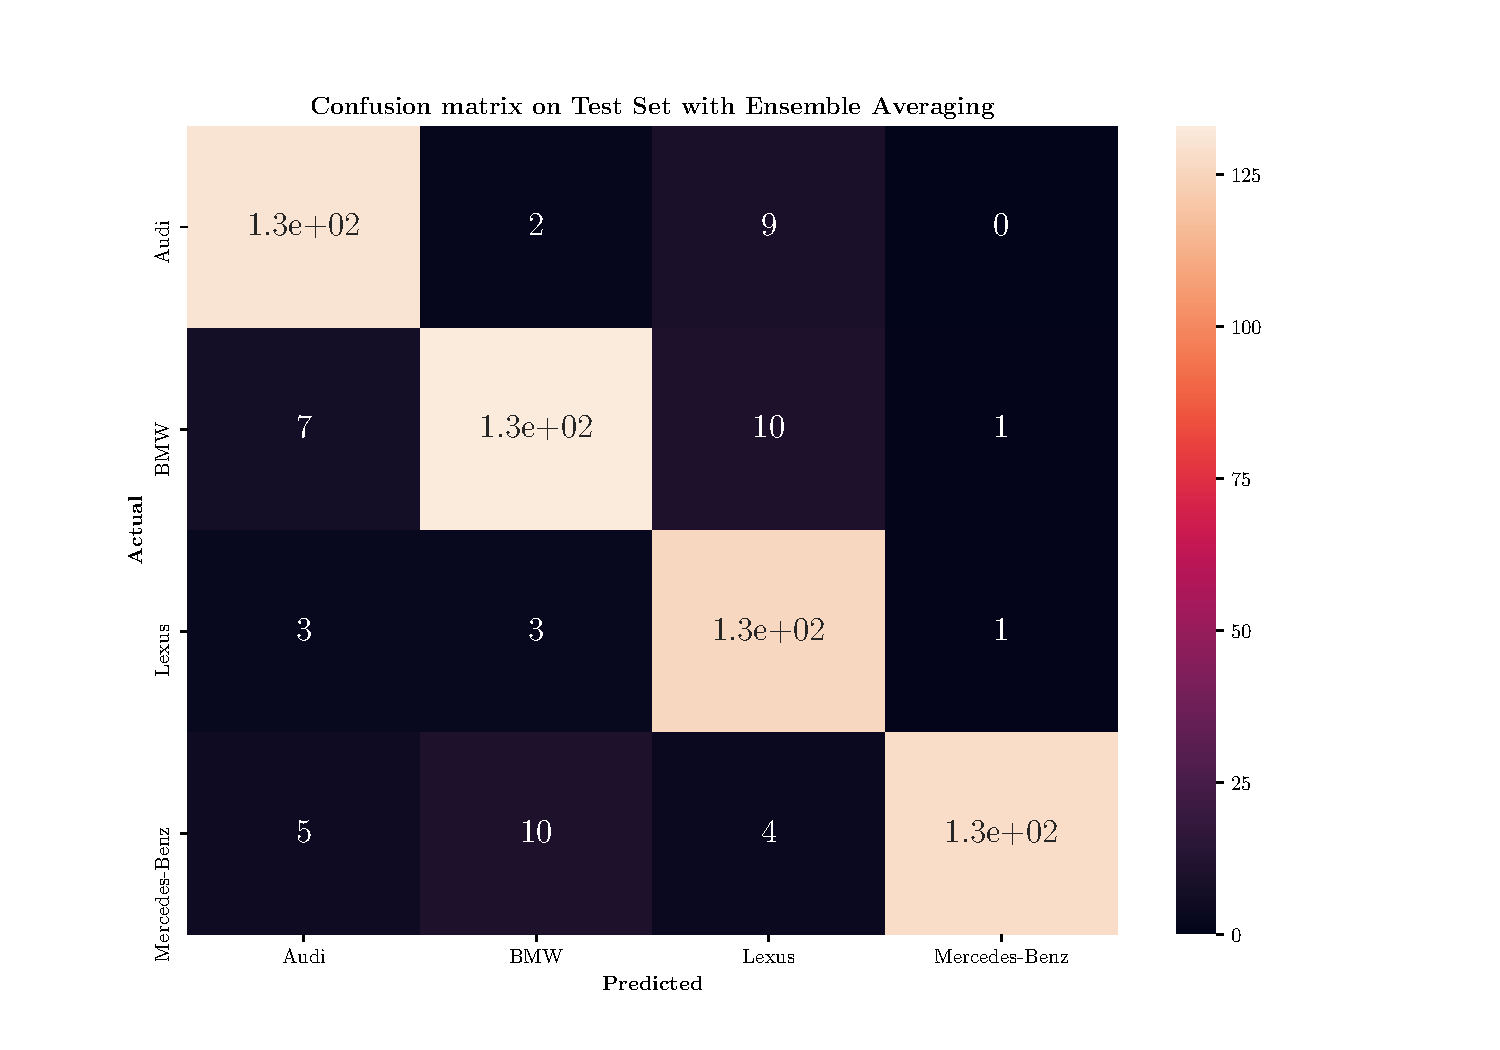
\includegraphics[scale=0.32]{main_25_multiclass_00_confusion_matrix.pdf}
    \caption{Confusion matrix on test set with ensemble averaging}
    \label{fig:confmat}
\end{figure}

\section{Conclusion and future work} \label{section:conclusion}
\textit{The Car Connection} dataset is a promising new dataset. With some cleaning effort, it was possible to exploit this dataset for image classification purposes. After benefiting from some extensive filtering in the future, the TCC dataset will then be mature enough for experimentation with more challenging classification tasks. In this work, it has proved to be a suitable dataset for binary and multi-class classification according to car brand. It is recommended to add bounding boxes to annotate the exact location of the cars in the dataset's images in future work. This will help in filtering out irrelevant background pixels in the pre-processing stage before the training stage.

For the arguably simple task of classifying car images between two brands, relatively shallow networks have been successfully trained to give a test accuracy exceeding $92\%$. As an ensemble, these ConvNets have achieved an appreciable increase of at least $0.27\%$ in testing accuracy. Future work may focus on developing better classifiers to beat these benchmark figures.

In the context of the multi-class classification problem, our ConvNet-based classifiers had a testing accuracy of at least $85\%$ individually. When ensembled together, their resulting classification accuracy increased to $90\%$. These figure serve as the benchmark performance to beat in future work.

It is recommended to include more classes to be classified in the experiments. To compensate for the relatively small number of examples in some classes which causes an imbalance in the dataset, it is recommended to incorporate more extensive data augmentation techniques in future work. Transfer learning from more established architectures may be a suitable avenue to explore in future work.

The far more challenging task of classifying car images according to body type (sedan, hatchback, convertible, SUV) is recommended as future work once the dataset has overcome its teething problems. Classification according to body type is a fine-grained classification problem and is therefore an interesting topic of research.









\addtolength{\textheight}{-15cm}   % This command serves to balance the column lengths
                                  % on the last page of the document manually. It shortens
                                  % the textheight of the last page by a suitable amount.
                                  % This command does not take effect until the next page
                                  % so it should come on the page before the last. Make
                                  % sure that you do not shorten the textheight too much.

%%%%%%%%%%%%%%%%%%%%%%%%%%%%%%%%%%%%%%%%%%%%%%%%%%%%%%%%%%%%%%%%%%%%%%%%%%%%%%%%


%%%%%%%%%%%%%%%%%%%%%%%%%%%%%%%%%%%%%%%%%%%%%%%%%%%%%%%%%%%%%%%%%%%%%%%%%%%%%%%%

\begin{thebibliography}{99}
\bibitem{kagcatdog}
``{Kaggle Dogs Versus Cats Challenge}.''
  \url{https://www.kaggle.com/c/dogs-vs-cats}.
\newblock [Accessed: 2020-03-01].

\bibitem{simonyan2014very}
K.~Simonyan and A.~Zisserman, ``Very deep convolutional networks for
  large-scale image recognition,'' {\em arXiv preprint arXiv:1409.1556}, 2014.

\bibitem{7744550}
J.~{Fang}, Y.~{Zhou}, Y.~{Yu}, and S.~{Du}, ``Fine-grained vehicle model
  recognition using a coarse-to-fine convolutional neural network
  architecture,'' {\em IEEE Transactions on Intelligent Transportation
  Systems}, vol.~18, no.~7, pp.~1782--1792, 2017.

\bibitem{7535529}
H.~{Huttunen}, F.~S. {Yancheshmeh}, and {Ke Chen}, ``Car type recognition with
  deep neural networks,'' in {\em 2016 IEEE Intelligent Vehicles Symposium
  (IV)}, pp.~1115--1120, June 2016.
  
\bibitem{7891907}
Q.~{Hu}, H.~{Wang}, T.~{Li}, and C.~{Shen}, ``Deep cnns with spatially weighted
  pooling for fine-grained car recognition,'' {\em IEEE Transactions on
  Intelligent Transportation Systems}, vol.~18, no.~11, pp.~3147--3156, 2017.
  
\bibitem{liu2017monza}
D.~Liu and Y.~Wang, ``Monza: image classification of vehicle make and model
  using convolutional neural networks and transfer learning.''
 
\bibitem{krizhevsky2012imagenet}
A.~Krizhevsky, I.~Sutskever, and G.~E. Hinton, ``Imagenet classification with
  deep convolutional neural networks,'' in {\em Advances in neural information
  processing systems}, pp.~1097--1105, 2012.
  
\bibitem{Szegedy2015CVPR}
C.~Szegedy, W.~Liu, Y.~Jia, P.~Sermanet, S.~Reed, D.~Anguelov, D.~Erhan,
  V.~Vanhoucke, and A.~Rabinovich, ``Going deeper with convolutions,'' in {\em
  The IEEE Conference on Computer Vision and Pattern Recognition (CVPR)}, June
  2015.

\bibitem{valev2018systematic}
K.~Valev, A.~Schumann, L.~Sommer, and J.~Beyerer, ``A systematic evaluation of
  recent deep learning architectures for fine-grained vehicle classification,''
  in {\em Pattern Recognition and Tracking XXIX}, vol.~10649, p.~1064902,
  International Society for Optics and Photonics, 2018.

\bibitem{he2016deep}
K.~He, X.~Zhang, S.~Ren, and J.~Sun, ``Deep residual learning for image
  recognition,'' in {\em Proceedings of the IEEE conference on computer vision
  and pattern recognition}, pp.~770--778, 2016.

\bibitem{huang2017densely}
G.~Huang, Z.~Liu, L.~Van Der~Maaten, and K.~Q. Weinberger, ``Densely connected
  convolutional networks,'' in {\em Proceedings of the IEEE conference on
  computer vision and pattern recognition}, pp.~4700--4708, 2017.

\bibitem{KrauseStarkDengFei-Fei3DRR2013}
J.~Krause, M.~Stark, J.~Deng, and L.~Fei-Fei, ``3d object representations for
  fine-grained categorization,'' in {\em 4th International IEEE Workshop on 3D
  Representation and Recognition (3dRR-13)}, (Sydney, Australia), 2013

\bibitem{githubrepo}
N.~Gervais, ``Predicting car price from scraped data.''
  \url{https://github.com/nicolas-gervais/predicting-car-price-from-scraped-data}.
\newblock [Accessed 21 February 2020].

%\bibitem{7299023}
%L.~{Yang}, P.~{Luo}, C.~C. {Loy}, and X.~{Tang}, ``A large-scale car dataset
 % for fine-grained categorization and verification,'' in {\em 2015 IEEE
  %Conference on Computer Vision and Pattern Recognition (CVPR)},
  %pp.~3973--3981, 2015.

%\bibitem{kerasapplications}
%``{Keras Applications}.'' \url{https://keras.io/applications/}.
%\newblock [Accessed: 2020-03-01].

\bibitem{chollet2018deep}
F.~Chollet, {\em Deep Learning with Python}.
\newblock Manning, 2018.

\bibitem{keras}
``{Keras}.'' \url{https://keras.io}.
\newblock [Accessed: 2020-04-13].


\end{thebibliography}




\end{document}
